\begin{figure*}[t]
    \centering
    % \includegraphics[width=\linewidth]{figures/pdf_files/method_v2.pdf}
    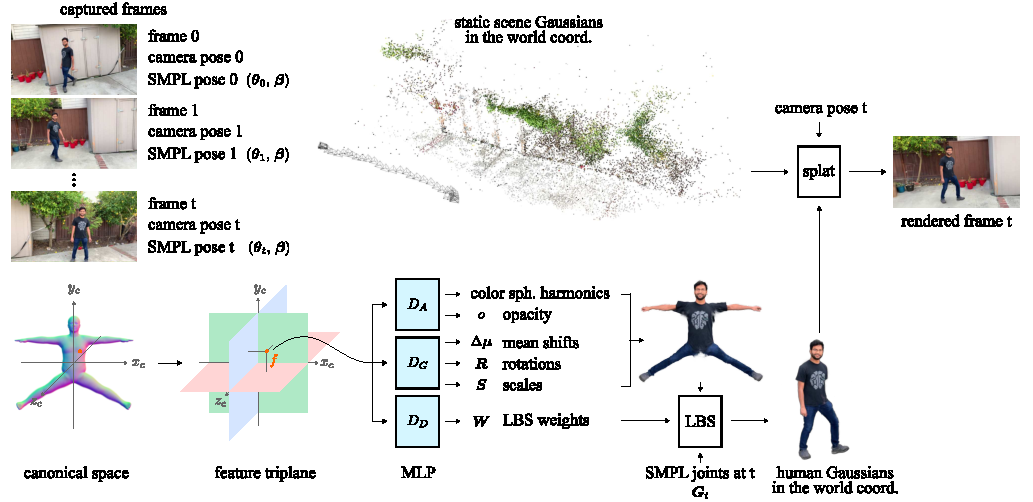
\includegraphics[width=\linewidth]{figures/method/method_small_v2.pdf}
    \vspace{-7mm}
    \caption{\textbf{\acronym overview.} Given a video with dynamic human and camera motions, \acronym recovers an animatable human avatar and synthesizes human and scene from novel view points. 
    Our method represents both the human and the scene as 3D Gaussians. The human Gaussians are parameterized by their mean locations in a canonical space and the features from a triplane. Three MLPs are used to estimate their color, opacity, additional shift, rotation, scale, and LBS weights to animate the Gaussians with given joint configurations.  
    %
    The human and the scene Gaussians are combined and rendered together with splatting. 
    %Our method first uses structure-from-motion and human pose estimation to obtain scene point-cloud, cameras, and SMPL parameters $\theta$. We use 3D Gaussians to represent the scene and human ($T$) in canonical coordinates. We then use GCN-based geometry, appearance, and deformation decoders to learn personalized Gaussian offsets, appearance, pose correctives $B_P(\theta)$ and linear blend skinning weights $W$. We then render the scene and deformed human 3D gaussians using differentiable Gaussian rasterization.
    } 
    \label{fig:overview}
    \vspace{-2ex}
\end{figure*}{}